\documentclass[9pt,twocolumn,twoside]{osajnl}
%% Please use 11pt if submitting to AOP
% \documentclass[11pt,twocolumn,twoside]{osajnl}



\usepackage[utf8]{inputenc}
\usepackage{soul}

\usepackage{siunitx}
\DeclareSIUnit\ppm{ppm}
\DeclareSIUnit\pixel{px}
\DeclareSIUnit\arb{AU}

\newcommand{\I}{\mathrm{i}}
\newcommand{\FE}{\textit{FE}}
\newcommand{\Sum}{\textit{Sum}}
\newcommand{\R}{\textit{R}}
\newcommand{\DefX}{\textit{DefX}}
\newcommand{\DefY}{\textit{DefY}}
\newcommand{\low}[1]{\textsubscript{#1}}


\journal{ao} % Choose journal (ao, aop, josaa, josab, ol, pr)

% See template introduction for guidance on setting shortarticle option
\setboolean{shortarticle}{true}
% true = letter / tutorial
% false = research / review article
% (depending on journal).

\title{A device for real-time monitoring of oil-in-water and suspended solids based on thermal lens spectrometry and light scattering}

\author[1,*]{Axel M. Lacapmesure}
\author[2]{Oscar E. Martínez}
\author[3]{Darío Kunik}

\affil[1]{Departamento de Física, Facultad de Ciencias Exactas y Naturales, Universidad de Buenos Aires, Pabellón I, Ciudad Universitaria, Intendente Güiraldes 2160, C1428EGA Ciudad Autónoma de Buenos Aires, Argentina}
\affil[2]{Laboratorio de Fotónica, Facultad de Ingeniería, Universidad de Buenos Aires, Av. Paseo Colón 850, C1063ACV Ciudad Autónoma de Buenos Aires, Argentina}
\affil[3]{YPF Tecnología S.A., Av. del Petróleo Argentino s/n, Berisso, 1923 Buenos Aires, Argentina}

\affil[*]{Corresponding author: alacapmesure@fi.uba.ar}

%% To be edited by editor
% \dates{Compiled \today}

%\ociscodes{(140.3490) Lasers, distributed feedback; (060.2420) Fibers, polarization-maintaining;(060.3735) Fiber Bragg gratings.}

%% To be edited by editor
% \doi{\url{http://dx.doi.org/10.1364/XX.XX.XXXXXX}}

\begin{abstract}
A novel system for simultaneous monitoring of both oil-in-water and suspended solids based on thermal lens spectroscopy and forward light scattering is presented. The technique measures the concentration of dissolved hydrocarbons and simultaneously detects single oil droplets and suspended particles separately. The device was tested with injection water from an on-field water treatment plant, and hydrocarbon concentrations were measured with a precision better than \SI{5}{\percent} in the range up to \SI{100}{\ppm}, reaching resolutions as low as \SI{0.02}{\ppm}. Particle detection was tested on artificial samples of polystyrene spheres acting as absorption and scattering centers, which simulated oil droplets and suspended solids respectively. We show that particles of different sizes are distinguished and their concentrations were determined in the range up to \SI{3000}{particles\per\milli\litre}.
\end{abstract}

\setboolean{displaycopyright}{true}

\begin{document}

\maketitle



\section{Introduction}
\label{Introduction}

Improved oil recovery techniques allows to enhance oil-production rate and extend the productive life of the oil well by artificially increasing reservoir pressure when its natural pressure declines. Secondary recovery techniques typically relies on water injection into the reservoir while tertiary recovery also incorporates chemical components (such as polymers or surfactants) in order to increase oil mobility. In all these projects, maintaining high injectivities over long periods of time is extremely important. With the increasing stream of oilified-produced waste water and the tightening of environmental regulations, produced water reinjection has become one of the best options to manage large volumes of waste water in an economically attractive and environmentally safe way \cite{Furtado2005,Souza2005,Abou-Sayed2007}. However, even after water treatment, the complexity of produced water composition leads to important difficulties for injection processes regarding plugging, corrosion and permeability impairment among other problems.

Produced water contains a complex variety of dissolved and particulate organic and inorganic chemicals, and its composition varies widely between different wells and also within well lifetime. Produced water compounds includes inorganic salts, metals, radioisotopes, chemicals used in the production systems, and a variety of organic chemicals \cite{Lee2011,Stephenson1992}. In untreated produced water, both aromatic and aliphatic hydrocarbons are present at concentrations up to \SI{800}{} parts per million mass/mass (\si{ppm}). The lightest hydrocarbons (mostly one-ring aromatic compounds) forms an homogeneous phase (dissolved oil) while the rest are present as oil droplets (dispersed oil) with sizes in the range \SI{1}{}--\SI{100}{\micro\metre} or even larger. Produced water also contains suspended solids (formation sands and clays or hydraulic fracturing proppants) with sizes within \SI{0.1}{\micro\metre}--\SI{1}{\milli\metre} range \cite{Stewart2011B,Cavallaro2000,Deng2009}. In water treatment plants, several methods are employed to extract undesired components from produced water before reinjection. However, depending on treatment efficacy, treated water may still contain both hydrocarbons and suspended solids at concentrations up to \SI{100}{\ppm} and with droplet/particle sizes up to \SI{10}{\micro\metre} or even bigger.

It has been found that induced injectivity decrease is more severe when both oil droplets and suspended solids are present in injection water because they interact jointly with the porous medium leading to particle deposition, pore bridging and internal or external cake formation \cite{Bennion1998,Chaveteau1998,Reousseau2008,Ali2009}. In all cases, the ratio between particle size and pore throat and the particle and oil concentrations are critical parameters since they have an important influence on the magnitude and time scale of permeability reduction \cite{vanderBroek1999,Ali2007,Buret2010}. This makes water quality analysis a key element for prediction and control of injectivity impairment and for the evaluation of water treatment processes, and online monitoring becomes a requirement for process trending and premature detection of process deviation In the last decades, new and fast techniques based on optical phenomena that does not requires sophisticated sample treatment were developed and implemented in oil industry, with some of them currently available in the market. Below we summarize the most noteworthy examples and some of the difficulties they present.

%Water quality analysis typically combines mechanical separation and/or chemical extraction techniques with physically or chemically based concentration measurements. Since these analysis demand long times (as long as several weeks) until results are available, new methods compatible with online monitoring are required for process trending and premature detection of process deviation. In the last decades, new and fast techniques based on optical phenomena that does not requires sophisticated sample treatment were developed and implemented in oil industry, with some of them currently available in the market. %Below we summarize the most noteworthy examples with some of the difficulties they present.

Scattering based methods detects the angular distribution of light scattered by oil droplets and other suspended particles contained in the sample. These systems don't account for dissolved hydrocarbons and showed difficulties to differentiate suspended particles of same size but different composition \cite{He2003}. Fluorescence based methods detect the fluorescence emission from aromatic components in the sample when it is irradiated with UV light. In this case the sensitivity is highly dependent on the relation between aromatics hydrocarbons and the rest of the oil components \cite[ch. 4]{Parker1987}, and both competing electronic decay processes and quenching alters the overall response at different concentration levels, thus introducing nonlinearities \cite{Downare1995}. Similarly a surface enhanced Raman scattering sensor was proposed for detection of polyciclic aromatic carbons such as anthracene and pryrene \cite{Kolomijeca2011}, but this method is also dependent of the relative concentration of aromatics hydrocarbons. Additionally some methods based on photoacustic sensors and UV/NIR light absorption were reported, but none has shown reliable at concentrations lower than \SI{50}{\ppm} \cite{Freeborn1998,He2003}. In all cases, none of the proposed methods allows for a separated characterization of both suspended solids and oil concentrations.

\hl{[RESUMIR Y AGREGAR SECTIONING]} In this work we present and discuss a novel water quality monitoring system for both oil-in-water and suspended solids measurement based on thermal lens spectrometry and forward light scattering. The device comprises a thermal lens spectrometer with a collinear pump and probe beam configuration. Both the power of the thermal lens and the optical transmission of the probe beam are measured. Transmission signal provides information about both absorbing (i.e. hydrocarbons) and scattering (i.e. suspended solids and oil droplets) components of the sample, while thermal lens signal only provides information about absorbing components, thus allowing to measure the concentration of dissolved oils as well as to detect oil droplets and suspended solids separately. The device can be incorporated into injection flowlines to be used as an online monitoring system.



\subsection{Thermal lens and focus error signal}

Techniques for sample characterization based on thermal lens effects had been extensively developed since the first report of thermal lens effect by Gordon in 1965 \cite{Gordon1965}, leading to some of the most sensitive methods for thermophysical and chemical analysis, such as thermal lens spectroscopy (TLS) \cite{Franko2010,Liu2016}. This technique is based on the measurement of the optical lens induced in an irradiated sample by the absorption of light and subsequent heating. Its application on chemical analysis is possible since the power of the lens depends on the concentration of absorbing components, and absorbances as low as \SI{7}{\arb} can be detected \cite{Proskurnin2015}. Thermal lens spectroscopy was successfully used on homogeneous media for chemical trace detection \cite{Sikovec1996,Franko2010}, while theoretical and experimental studies have been conducted to measure characterize colloidal suspensions \cite{Brusnichkin2007,Marcano2011,Rusconi2004}. In the context of thermal lens microscopy, single particle detection was also theoretically studied \cite{Selmke2015} and experimentally demonstrated for both micrometer-sized particles \cite{Harada1995,Andika2010} and metallic nanoparticles \cite{Berciaud2005,Gaiduk2010}.
%hence allowing detection of absorbances as low as \SI{d-7}{\arb} \cite{Proskurnin2015}. In comparison to other optical methods, thermal lens based techniques are intrinsically less sensitive to scattering effects, making it ideal for characterization of heterogeneous samples or colloidal suspensions while also offering diverse and versatile configurations in order to exploit the photochemical properties of the sample. The theory of thermal lens signal in homogeneous sample was vastly studied \cite{Bialkowski2019}. Thermal lens spectrometry was also applyied to characterize colloidal media [REFERENCIAS]. Single particle detection was demonstrated in the context of thermal lens microscopy, Theory of thermal lens signal arising from a single absorber was also studied \cite{Selmke2012}. %Thermal lens spectrometry has proven useful in diverse high sensitivity chemical trace detection and analysis \cite{Sikovec1996,Franko2010}, and it can also be coupled to chemical separation systems or microfluidic injection systems for enhanced selectivity \cite{Liu2016}. \\

The theory of thermal lens generation on homogeneous media is widely discussed in literature \cite{Bialkowski2019}. In a typical TLS experiment, a high-power pump beam is focused on the sample under study. The absorption of a fraction of the pump beam energy within the sample locally increases the temperature in the medium, thus generating a refractive index gradient. This thermal lens is detected by measuring the defocusing (if the sample is an aqueous medium, due to the negative sign of the thermo-optic coefficient of water) of a second, low-power, collinear probe beam. The pump beam intensity is usually modulated to allow a phase-sensitive detection with a Lock-In amplifier. Since the power of the thermal lens is proportional to the total energy absorbed, this methods allows to perform high-sensitivity absorbance measurements. Single absorbing particles may also be detected due to the generation of micro-lenses around the particle. In this case, the induced refractive index has a long-ranged profile with a characteristic length $R_{th} = \sqrt{2 \kappa / \Omega C}$, where $\kappa$ and $C$ are the mediums' heat conductivity and heat-capacity per unit volume respectively, and $\Omega$ is the pump beam's modulation frequency \cite{Selmke2015}.

%To generate the thermal lens, both beams are focused on a sample contained in a flourometer cuvette. Along the beam propagation through the sample, the pump beam energy is partially absorbed and dissipated as heat, thus locally increasing the temperature of the medium and generating a refractive index profile. If the temperature elevation is smooth enough, the refractive index profile forms an optical lens that defocuses the probe beam due to the negative sign of the thermo-optic coefficient of water. In the low-absorption regime, the power of this thermal lens is proportional to the total energy absorbed, hence allowing to perform high-sensitivity absorbance measurements by characterizing the probe beam defocusing.

The thermal lens signal is typically obtained by measuring the far-field, on-axis probe beam's intensity using a photodiode behind a small pinhole. An alternative and highly sensitive method consists on characterizing the defocusing of the probe beam by measuring a focus error (\FE{}) signal from a four-quadrant photodetector \cite{Domene2017, ZaldivarEscola2019}. In this method, two cylindrical lenses are located at a distance $s$ after the sample and separated a distance $d$ from each other. The axes of the lenses are placed perpendicular to each other so the probe beam becomes astigmatic. The beam ellipticity is then measured with a four-quadrant photodetector, which consists on an array of four identical photodiodes (A, B, C and D). This is done using the \FE{} signal obtained by comparing each single photodiode signal: $\FE{} = (A+C)-(B+D)$.

Figure \ref{fig:FESignal} shows the value of the \FE{} signal along the propagation of the astigmatic probe beam. Initially, the detector is placed at the intermediate plane $z_c$ where the beam is circular, so the \FE{} signal is zero in the absence of a sample. When a thermal lens appears, the probe beam is defocused and the position $z_c$ is displaced along the optical axis, thus generating a nonzero \FE{} signal. In the case of an intensity modulated pump beam and in the limit of a low power thermal lens, the \FE{} signal oscillates around a CW value with an amplitude proportional to the thermal lens power. By normalizing the \FE{} signal with the total intensity transmitted through the sample $\Sum{} = A+B+C+D$, the \FE{} signal is independent of the probe beam's transmission fluctuations. A notable difference between this method and the on-axis intensity measurement is that, for a suitable choice of the parameter $s$, an absorbing particle located anywhere in the sample will generate a nonzero \FE{} signal, while the on-axis intensity signal has a zero point when the particle is located at the probe beam's waist. In addition, the \Sum{} signal can be used for traditional transmission measurements.

\begin{figure}[ht]
	\centering 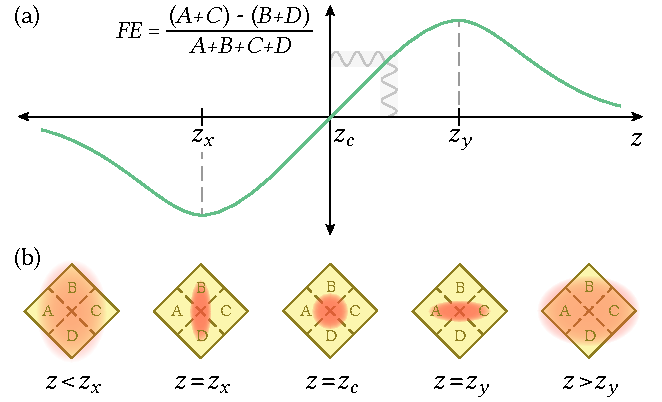
\includegraphics[width=.46\textwidth]{figures/FESignal.pdf}
	\caption{(a) \FE{} signal response as a function of the four-quadrant photodetector position along optical axis and (b) the astigmatic probe beam incident on four-quadrant detector at some cases. $z_x$ and $z_y$ indicates the beam waist location for each axis. An oscillating thermal lens moves the beam waists along the optical axis and thus generates an oscillating \FE{} signal (depicted by sinusoidal lines).}
	\label{fig:FESignal}
\end{figure}

%Subsequently the probe beams enters the focus error detection system, where both the change of focus and its transmitted power are measured. The system comprises a pair of cylindrical lenses whose axes are oriented orthogonally, therefore creating an astigmatic focused beam with waists in the horizontal and vertical directions at different planes. There is an intermediate plane where the beam is circular, and the presence of a thermal lens that defocuses the probe beam moves this plane along the optical axis. A four-quadrant photodiode was used to measure the beam ellipticity through generation of a focus error \FE{} signal \cite{Domene2017, ZaldivarEscola2019}. Additionally the total transmitted power is measured by summing the signals of all quadrants, allowing traditional measurements of the sample transmission to obtain its extinction coefficient. Normalizing \FE{} with the transmitted power leads this signal to respond only to beam geometry independently of its intensity, and thus characterizing the probe beam defocusing: \FE{} is zero when placed in the plane where the beam is circular, but in presence of a thermal lens, the beam on that plane becomes elliptical and leads to a nonzero \FE{} signal. \\

%In this work we present and discuss a novel water quality monitoring system for both oil-in-water and suspended solids measurement based on thermal lens spectrometry and forward light scattering. The device comprises a thermal lens spectrometer with a pump and probe beam configuration where both the power of the thermal lens and the optical transmission of the probe beam are measured. Transmission signal provides information about both absorbing (i.e. hydrocarbons) and scattering (i.e. suspended solids and oil droplets) components of the sample, while thermal lens signal only provides information about absorbing components, thus allowing to measure the concentration of dissolved oils as well as to detect oil droplets and suspended solids separately. Along our work the device was tested with water samples from on-field water treatment facilities and also with artificial colloidal suspensions made for controlled tests. The whole system allowed a continuous and fast characterization of the sample with measurement duration of about \SI{200}{\second}, and since sample preparation isn't required and its configuration is compatible with a flow-through system, the device proves ideal for usage as an online monitor that can be incorporated into injection flowlines.








\section{Experimental}
\label{Experimental}

Our device consists in a thermal lens spectrometer with a dual collinear beam configuration and a focus error system with phase-sensitive detection. For an efficient oil-in-water detection, a high background contrast in the photothermal and transmission signals is desired, which implies a high contrast in the absorption and scattering properties between oil and water. Optical absorption of crude oil varies widely between different types and in the visible region exhibits an exponential decrease with increasing wavelength which covers a range from \SI{500}{\per\centi\metre} down to \SI{50}{\per\centi\metre} \cite{OilCatalogue2005}. Also, the real part of its refractive index ranges between different oils \SI{1.46}{} and \SI{1.53}{} \cite{Otremba2000} without major variations at different wavelengths. Therefore we chose a \SI{532}{\nano\metre} wavelength where the absorption coefficient of oil is typically \SI{6}{} to \SI{7}{} orders of magnitude larger than for water, and also high-power lasers are available.

The power of the thermal lens is strongly enhanced by focusing the pump beam only up to the point where its confocal distance $2 z_R$ is comparable to the path length of the sample cell $L$. Also, the probe beam's mode should be smaller than or comparable to the pump beam's mode within the sample so it propagates within the perturbed refractive index region. Since a highly focused probe beam is less sensitive to the defocusing from a thermal lens, the confocal lengths of both beams were chosen to be similar to the path length of the sample cell.

% intensity modulated pump beam and a low-power, CW probe beam. The configuration consists of two main distinct sections: the thermal lens generation sector, which essentially comprises the lasers and the sample, and the focus error detection system, through which simultaneous measurement of both the thermal lens power and the optical transmission of the probe beam were made \cite{Domene2017}.

%To generate the thermal lens, both beams are focused on a sample contained in a flourometer cuvette. Along the beam propagation through the sample, the pump beam energy is partially absorbed and dissipated as heat, thus locally increasing the temperature of the medium and generating a refractive index profile. If the temperature elevation is smooth enough, the refractive index profile forms an optical lens that defocuses the probe beam due to the negative sign of the thermo-optic coefficient of water. In the low-absorption regime, the power of this thermal lens is proportional to the total energy absorbed, hence allowing to perform high-sensitivity absorbance measurements by characterizing the probe beam defocusing.
%In order to achieve an efficient oil-in-water detection it is necessary to choose a pump wavelength that gives a high contrast between absorption from oil and water. We chose a \SI{532}{\nano\metre} wavelength at which the absorption coefficient of oil is typically \SI{6}{} to \SI{7}{} orders of magnitude larger than for water, and also high-power lasers are available.

% Subsequently the probe beams enters the focus error detection system, where both the change of focus and its transmitted power are measured. The system comprises a pair of cylindrical lenses whose axes are oriented orthogonally, therefore creating an astigmatic focused beam with waists in the horizontal and vertical directions at different planes. There is an intermediate plane where the beam is circular, and the presence of a thermal lens that defocuses the probe beam moves this plane along the optical axis. A four-quadrant photodiode was used to measure the beam ellipticity through generation of a focus error \FE{} signal \cite{Domene2017, ZaldivarEscola2019}. Additionally the total transmitted power is measured by summing the signals of all quadrants, allowing traditional measurements of the sample transmission to obtain its extinction coefficient. Normalizing \FE{} with the transmitted power leads this signal to respond only to beam geometry independently of its intensity, and thus characterizing the probe beam defocusing: \FE{} is zero when placed in the plane where the beam is circular, but in presence of a thermal lens, the beam on that plane becomes elliptical and leads to a nonzero \FE{} signal. \\

\begin{figure*}[ht]
	\centering 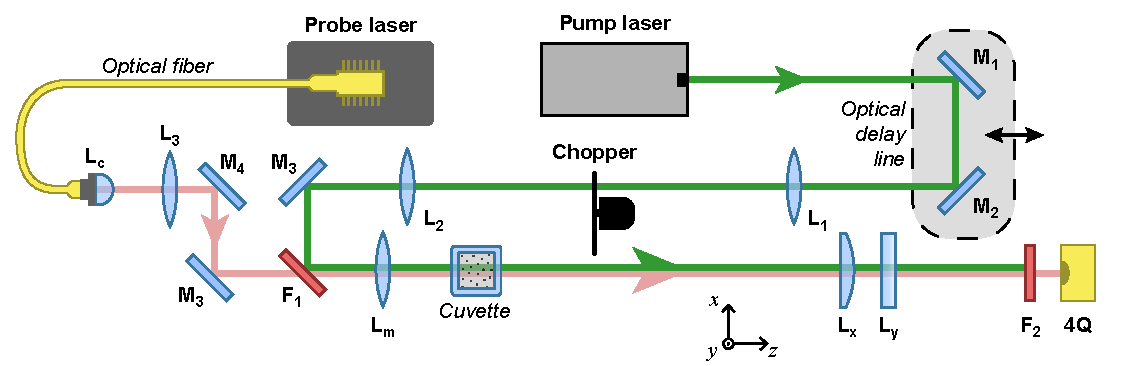
\includegraphics[width=\textwidth]{figures/Setup.pdf}
	\caption{Experimental setup. \textbf{M\low{1} to M\low{5}:} mirrors for beam alignment. \textbf{L\low{c}:} probe collimating lens. \textbf{L\low{1} to L\low{3}:} pump and probe optics, in addition with \textbf{L\low{m}}. \textbf{F\low{1} and F\low{2}:} \SI{700}{\nano\metre} longpass filter for beam coupling and pump filtering respectively. \textbf{L\low{x} and L\low{y}:} cylindrical lenses. \textbf{4Q:} four-quadrant photodiode.}
	\label{fig:Experimental}
\end{figure*}

Figure \ref{fig:Experimental} shows a simplified diagram of the experimental setup. The sample was contained in a PMMA fluorometer cuvette with a \SI{10}{\milli\metre} optical path length. The pump laser was a frequency doubled Nd:YAG laser \emph{Coherent} model \emph{Compass 315M-100} with a \SI{100}{\milli\watt} maximum output power at a \SI{532}{\nano\metre} wavelength. The pump beam was focused on the sample by a \SI{50}{\milli\metre} focal length lens $\mathrm{L_m}$. The pump beam's waist radius in the sample was $w_0^{(e)} = \SI{55}{\micro\metre}$, its confocal parameter was $2z_R^{(e)} = \SI{50}{\milli\metre}$ and the illuminated volume was \SI{0.1}{\milli\metre^3}. The position of the pump waist within the sample was controlled by an optical delay line constituted by mirrors $\mathrm{M_1}$ and $\mathrm{M_2}$ on a translation stage along with a 1X telescope constituted by lenses $\mathrm{L_1}$ and $\mathrm{L_2}$. A longpass filter $\mathrm{F_1}$ was used for collinear propagation.

The probe laser was a fiber-coupled laser diode \emph{QPhotonics} model \emph{QFLD-780-100S}, which provided a high quality Gaussian beam with a power of \SI{500}{\micro\watt} at a \SI{780}{\nano\metre} wavelength. The probe beam was firstly collimated by the lens $\mathrm{L_c}$ and then both lenses $\mathrm{L_3}$ and $\mathrm{L_m}$ were used to focus the beam on the sample, obtaining a beam's waist radius $w_0^{(p)} = \SI{33}{\micro\metre}$ and a confocal length $z_R^{(p)} = \SI{11.5}{\milli\metre}$ within the sample. 

The pump beam was intensity modulated by a rotating disc chopper. The election for the chopping frequency $\Omega$ poses a compromise between increasing the photothermal signal level (which enhances at lower frequencies due to a higher absorbed energy per cycle) and improving the time response of the detection (which is faster for lower time constants of the Lock-In amplifier). With those considerations we chose a frequency $\Omega = \SI{350}{\hertz}$, which also was much faster than the characteristic times of heat transfer by convection and diffusion processes, hence simplifying the thermal lens dependence by neglecting these effects. In addition, a point heat source within an aqueous sample would generate a thermal lens of size $R_{th} = \SI{30}{\micro\metre}$ comparable to the probe beam's waist radius, which is a requirement for single particle detection.


%The pump beam focusing optics was chosen to obtain a confocal parameter on the sample similar to the optical path of the cuvette. In order to minimize aberrations introduced by the edges of the thermal lens, the probe beam focusing optics was chosen to maximize the path length over which the probe beam was smaller than the pump beam. Altogether, this led to beam waists of \SI{55}{\micro\metre} for the pump beam and of \SI{33}{\micro\metre} for the probe beam. To control the displacement between both waists along the optical axis, the pump beam passed through a simple optical delay line comprised of two mirrors on a translation stage.

The focus error detection system comprised two \SI{75}{\milli\metre} focal length cylindrical lenses and a \SI{1}{\milli\metre^2} total active area four-quadrant photodetector. The system has two free parameters, namely the separation between the lenses $d$ and the distance from the lenses to the sample $s$. We chose these parameters by optimizing the sensitivity of the \FE{} signal in the presence of a thermal lens. To do so, the beam propagation and the \FE{} signal as a function of ${d,s}$ were numerically simulated, and the optimal configuration within mechanical limitations was chosen. Afterwards the detector was positioned on the plane where the probe beam was circular. In practice, the \FE{} signal was obtained from the signal of all quadrants by a series of summing op-amps circuits and then acquired and processed by a PCI lock-in amplifier \emph{Anfatec} model \emph{AMU 2.4} in order to extract the harmonic component at the pump modulation frequency. Additionally the signal from each quadrant was acquired by a 16 bits, \SI{1}{\mega\hertz} bandwidth, PCI DAQ board \emph{IOtech} model \emph{DaqBoard/3001}. This allowed to measure the total transmitted power by summing the signals from all quadrants through software and hence to normalize the \FE{} signal, and also to generate additional auxiliary signals. \\

With our prior understanding of the system we can already anticipate the signals responses in the presence of a sample of injection water. On the one hand, the absorbing components dissolved in water along with water itself will contribute to generate a thermal lens distributed over the irradiated volume, therefore increasing the thermal lens channel base level and decreasing the transmission channel base level due to bulk light absorption. We extract the absorption base level by computing the mode of the normalized thermal lens signal instead of its average since \FE{} signal fluctuations are asymmetric. On the other hand, suspended particles such as solids or oil droplets with sizes comparable to the beams waist will pass through the beams and alter the response previously described. If the particle does not absorbs the pump radiation, it will act as a scattering center and momentarily decrease the transmitted power, which will be observed as a negative peak in the transmission channel. If the particle does absorb the pump radiation it will also generate a thermal lens located around itself and thus defocus the probe beam even more, which will be observed as an additional positive peak in the thermal lens channel. To detect the contribution on each signal from suspended particles we use a peak detection algorithm developed on \emph{Matlab} that compares the signal fluctuations with those obtained with a sample of pure demineralized water, obtaining a time series of positive or negative peaks for each channel. In our work, particle detection was performed in a post-processing stage, but it can be conducted in real-time processing.

Our experiments were designed and conducted to study the system behavior considering the above discussed preliminary analysis. To do so, we had two master samples taken from an injection well facility located in Comodoro Rivadavia, Argentina. The first one, which we will refer as IW100, is a sample of the injection water that consists on treated produced water, and had oil-in-water concentration of at least \SI{100}{\ppm}. The second one, which we will refer as IW10, is a sample of the water used for manufacturing of polymers used in chemically-enhanced extraction. It consists of the same injection water with further treatment and had a oil concentration of less than \SI{10}{\ppm}. The concentration values were given by the company that took the samples and performs water quality analysis periodically on this well. Additionally, to study the system behavior with controlled samples when analyzing the suspended particles, we prepared artificial colloidal samples of microspheres suspended on demineralized water. To simulate suspended solids we used polystyrene spheres with a diameter of \SI{6}{\micro\metre}, while to simulate oil droplets we used polystyrene spheres dyed with a red pigment (thus absorbing at a \SI{532}{\nano\metre} wavelength) with diameters of \SI{6}{\micro\metre} and \SI{2}{\micro\metre}. We will refer to each master sample made as PS6 for the \SI{6}{\micro\metre} diameter undyed polystyrene spheres, and as PSD6 and PSD2 for the \SI{6}{\micro\metre} diameter and \SI{2}{\micro\metre} diameter polystyrene dyed spheres respectively. All spheres were manufactured by \emph{Phosphorex Inc.}








\section{Results and discussion}
\label{Results}

To study the system capability for characterizing dissolved components we performed serial dilutions of the IW100 and IW10 samples. First we progressively diluted IW100 on IW10, thus varying the oil concentration while preserving some of the water components. Secondly we diluted IW10 on demineralized water to extend the concentration range to lower values. For each iteration we performed a measurement with the same fixed parameters, namely lasers output power, acquisition length, lock-in and DAQ parameters, and then processed the data as above mentioned, obtaining the results plotted in figure \ref{fig:BulkAbsorption}.

\begin{figure}[t!]
	\centering 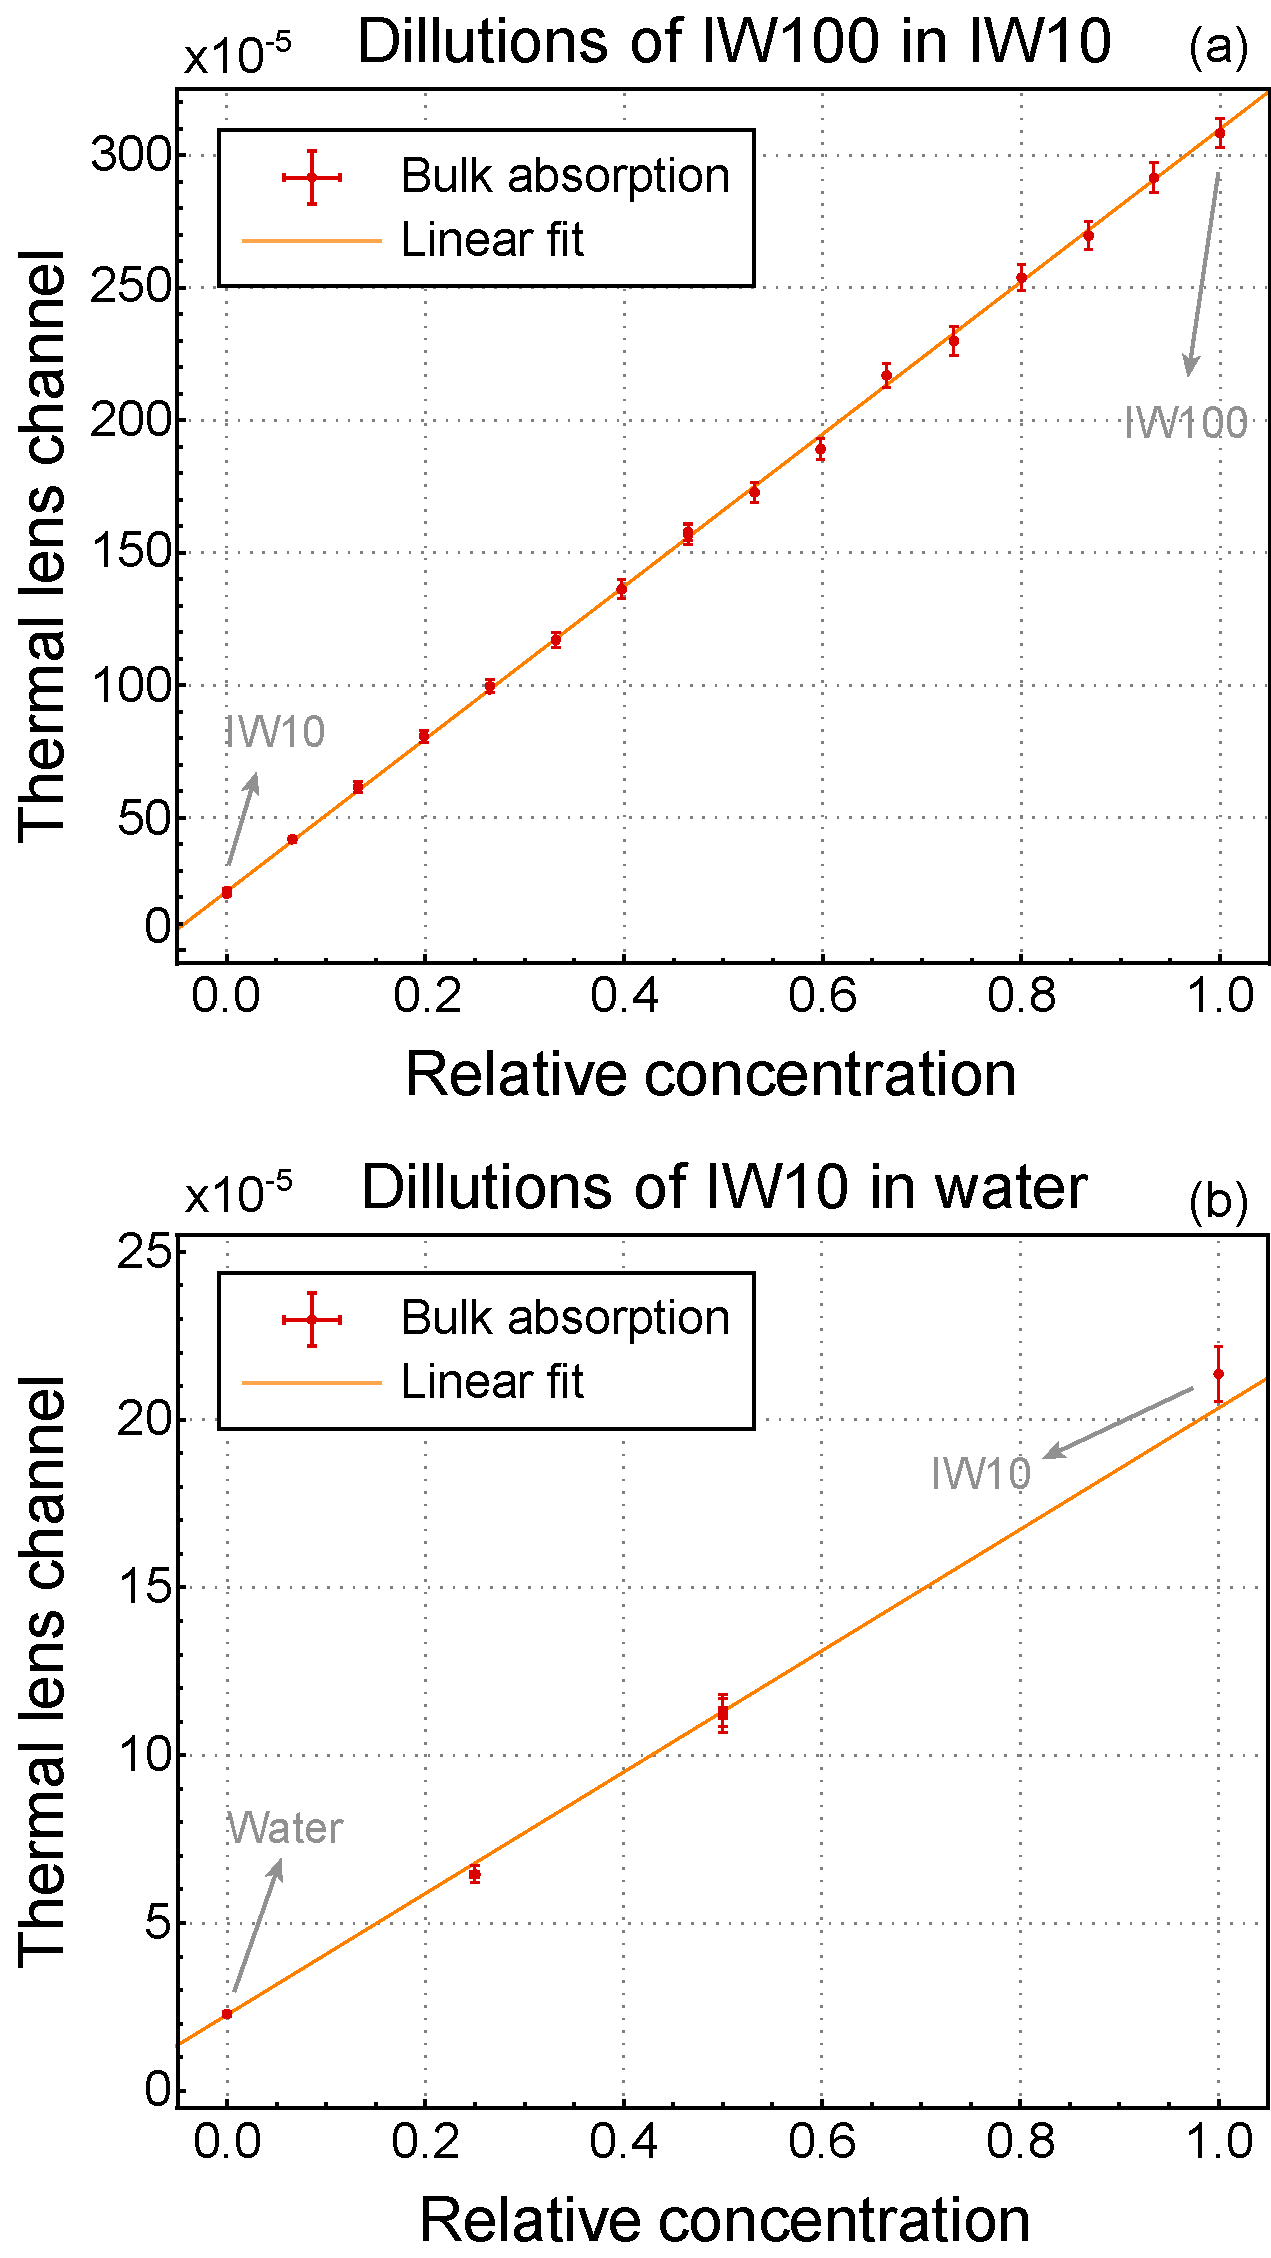
\includegraphics[width=.46\textwidth]{figures/IWvsC.pdf}
	\caption{Thermal lens signal from bulk absorption of dissolved components for serial dilutions of (a) IW100 on IW10 and (b) IW10 on demineralized water.}
	\label{fig:BulkAbsorption}
\end{figure}

The measurements for dilutions of IW10 on water allowed to study the performance of the device for injection water samples in the lowest absorption regime, recovering a linear response over the whole range of concentrations. A least squares linear regression was performed on the data, and from the adjusted slope it was possible to experimentally estimate the sensitivity of the device in therms of concentration by assuming an oil concentration of \SI{10}{\ppm} for the pure IW10 sample, resulting in a sensitivity of $\SI{1.8084(34)d-5}{\per\ppm}$ (note that \FE{} signal has no units after normalization with the transmission signal). If the actual concentration of the master sample would have been lower, our sensitivity would rise and therefore this value corresponds to a lower bound for the device sensitivity on these samples.

The ability to detect a certain amount of oil in the sample corresponds to the ability to distinguish its signal level from the background level due to absorption of pure water. Resolution is thus limited by both the contrast of water and oil absorption, which depends on the absorption properties specific of the oil, and the signal fluctuations, which comprises mainly the noise and the variations induced by inhomogeneities in the sample composition. The measurement uncertainty thus depends on both the lock-in time constant and the acquisition duration, improving for longer acquisitions since they allow a better reconstruction of the signal distribution and a more reliable calculation of the mode. We measured the variance of the mode as a function of these parameters and then take the resolution of the device as the variance for an acquisition length of \SI{200}{\s} and time constant of \SI{1}{\s}. We do so independently of the sample by taking into account only the fluctuations introduced by the system noise (i.e. without the fluctuations due to inhomogeneities in the sample composition), obtaining a resolution of \SI{0.02}{\ppm}.

Additionally, the dilutions of IW100 in IW10 allowed us to cover the range of concentrations of interest for most injection activities. In this range we again observed a linear response that gives the calibration coefficients for this well once the exact oil concentration of the master samples are known. In all cases the measurement precision, obtained by the same way as the above resolution but now taking into account all fluctuations, was better than \SI{5}{\percent}, being mostly limited by the fluctuations introduced by the sample inhomogeneous composition. Hence an oil concentration around \SI{10}{\ppm} could be determined with an uncertainty better than \SI{0.2}{\ppm} after proper calibration. \\

When studying the system capability for particles and emulsion characterization, firstly we calculated the peak series on both channels for each suspension of spheres in water and compared it with a demineralized water reference, which also showed some peaks due to the presence of suspended particles. We observed that the amount of peaks detected agreed with the expected behavior of the signals described in our preliminary analysis. The undyed spheres, which acted only as scattering centers, showed \SI{40}{} times more negative peaks detected than for water. We did not register any increase in peaks on the thermal lens channel, indicating not only the absence of absorption centers but also that the thermal lens signal is not affected by scattering losses. The dyed spheres showed a similar increase for both negative peaks in the transmission channel and positive peaks in the thermal lens channel, indicating the spheres acted as both scattering and absorption centers.

To study the magnitude of the effects introduced by particles, we compute the height $p$ of each peak relative to the base signal level due to the bulk absorption of the sample. Figure \ref{fig:PeakHistogram} shows an histogram of the peak relative heights for all samples registered at (a) the transmission channel and (b) the thermal lens channel. When comparing particles of different sizes, the negative peaks in transmission channel reveals that larger spheres produces a distribution of higher peaks. This is also shown by the calculated mean peak height, which was of \SI{19.9d-3}{} for the PSD6 sample and of \SI{17.5d-3}{} for the PS6 sample (absolute values of \SI{0.422}{\volt} and \SI{0.404}{\volt} respectively), while the PSD2 sample had a mean height of \SI{6.54d-3}{} (absolute height of \SI{0.140}{\volt}). As expected for the transmission channel, there isn't any significant difference between the distributions obtained for spheres of the same size, whether dyed or undyed, indicating that absorption losses are negligible in relation to the total incident power.

\begin{figure}[t!]
	\centering 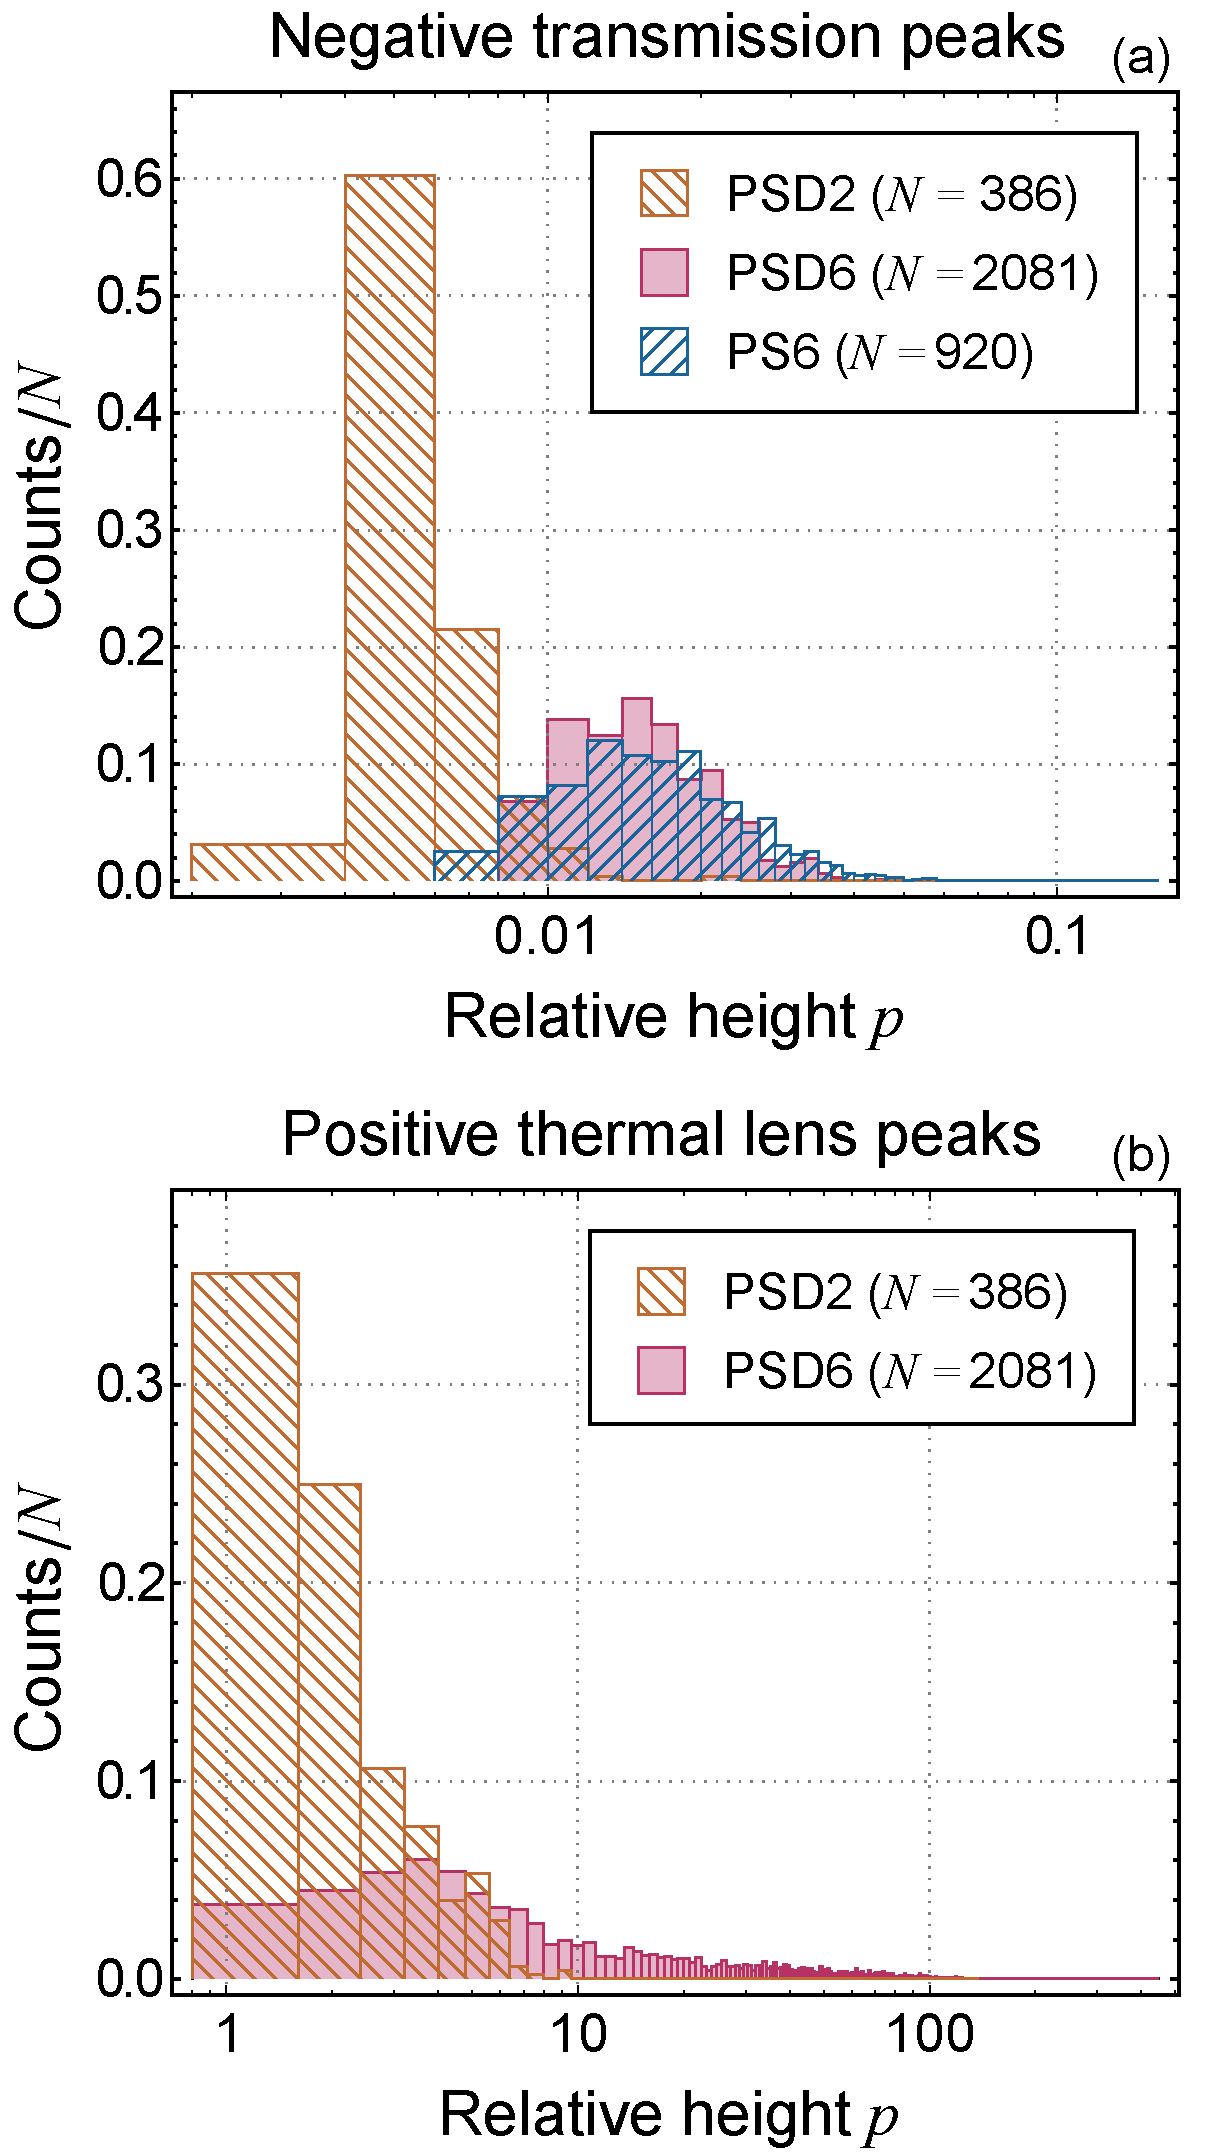
\includegraphics[width=.46\textwidth]{figures/PeakHeightDistribution.pdf}
	\caption{Histograms of relative peaks heights for (a) transmission channel and (b) thermal lens channel. On each case, counts are normalized to the total number of peaks detected $N$.}
	\label{fig:PeakHistogram}
\end{figure}

From figure \ref{fig:PeakHistogram} (b) we can make a similar analysis regarding the thermal lens channel, where we excluded the PS6 sample since it did not produce a significant amount of peaks in this signal. Here again we observe a distribution of peaks with larger heights for the suspension with bigger spheres, which is also consistent with the calculated mean peak heights of \SI{2.86}{} for PSD2 sample and \SI{24.8}{} for PSD6 sample (absolute heights of \SI{1.00d-4}{} and \SI{7.74d-4}{} respectively). Considering that the thermal lens channel is insensitive to scattering from a single particle, the information provided by both channels is complementary and allows to differentiate suspended solids and oil droplets not only by their absorption but also by their size, since the peak heights correlates with their scattering or absorption cross section depending on the channel. It should be noted that peak detection is much more improved on the thermal lens channel, where peak prominence is several orders of magnitude larger than in transmission channel. This is due to both the better signal-to-noise ratio of phase-sensitive detection and the choice for a pump wavelength in the water absorption minimum, resulting in a higher contrast and therefore an improvement in the characterization of absorbing components in the sample. \\

Particles concentration can be determined by studying the frequency of peaks. Assuming a suspension of ideal and statistically independent particles and for concentrations low enough to consider negligible the probability of finding one particle in the sampling volume, the passage of particles through the beams follows a Poisson statistics in which the interarrival time $\Delta$ between particles passing through the beams has a probability distribution
\begin{equation}
	P\left(\Delta > t\right) = \exp\left( -b t \right),
\label{eq:InterarrivalTimesPD}
\end{equation}
with $b$ being the reciprocal mean interarrival time, i.e. $\left\langle \Delta \right\rangle = 1/b$. We verified this behavior by computing the cumulative distribution probability of $\Delta$ for both the negative peaks of transmission channel and positive peaks of thermal lens channel, obtaining a probability distribution that agrees with \ref{eq:InterarrivalTimesPD} for values of $\Delta$ greater than the minimum interarrival time $\Delta_{min}$ our system could resolve. Here, $\Delta_{min}$ was limited mainly by the average peak width, the time constant of the lock-in amplifier and the fact that our system can't distinguish between one or many particles in the sampling volume, making our measurements valid only for concentrations low enough to neglect the case where multiple particles are present.

\begin{figure}[t!]
	\centering 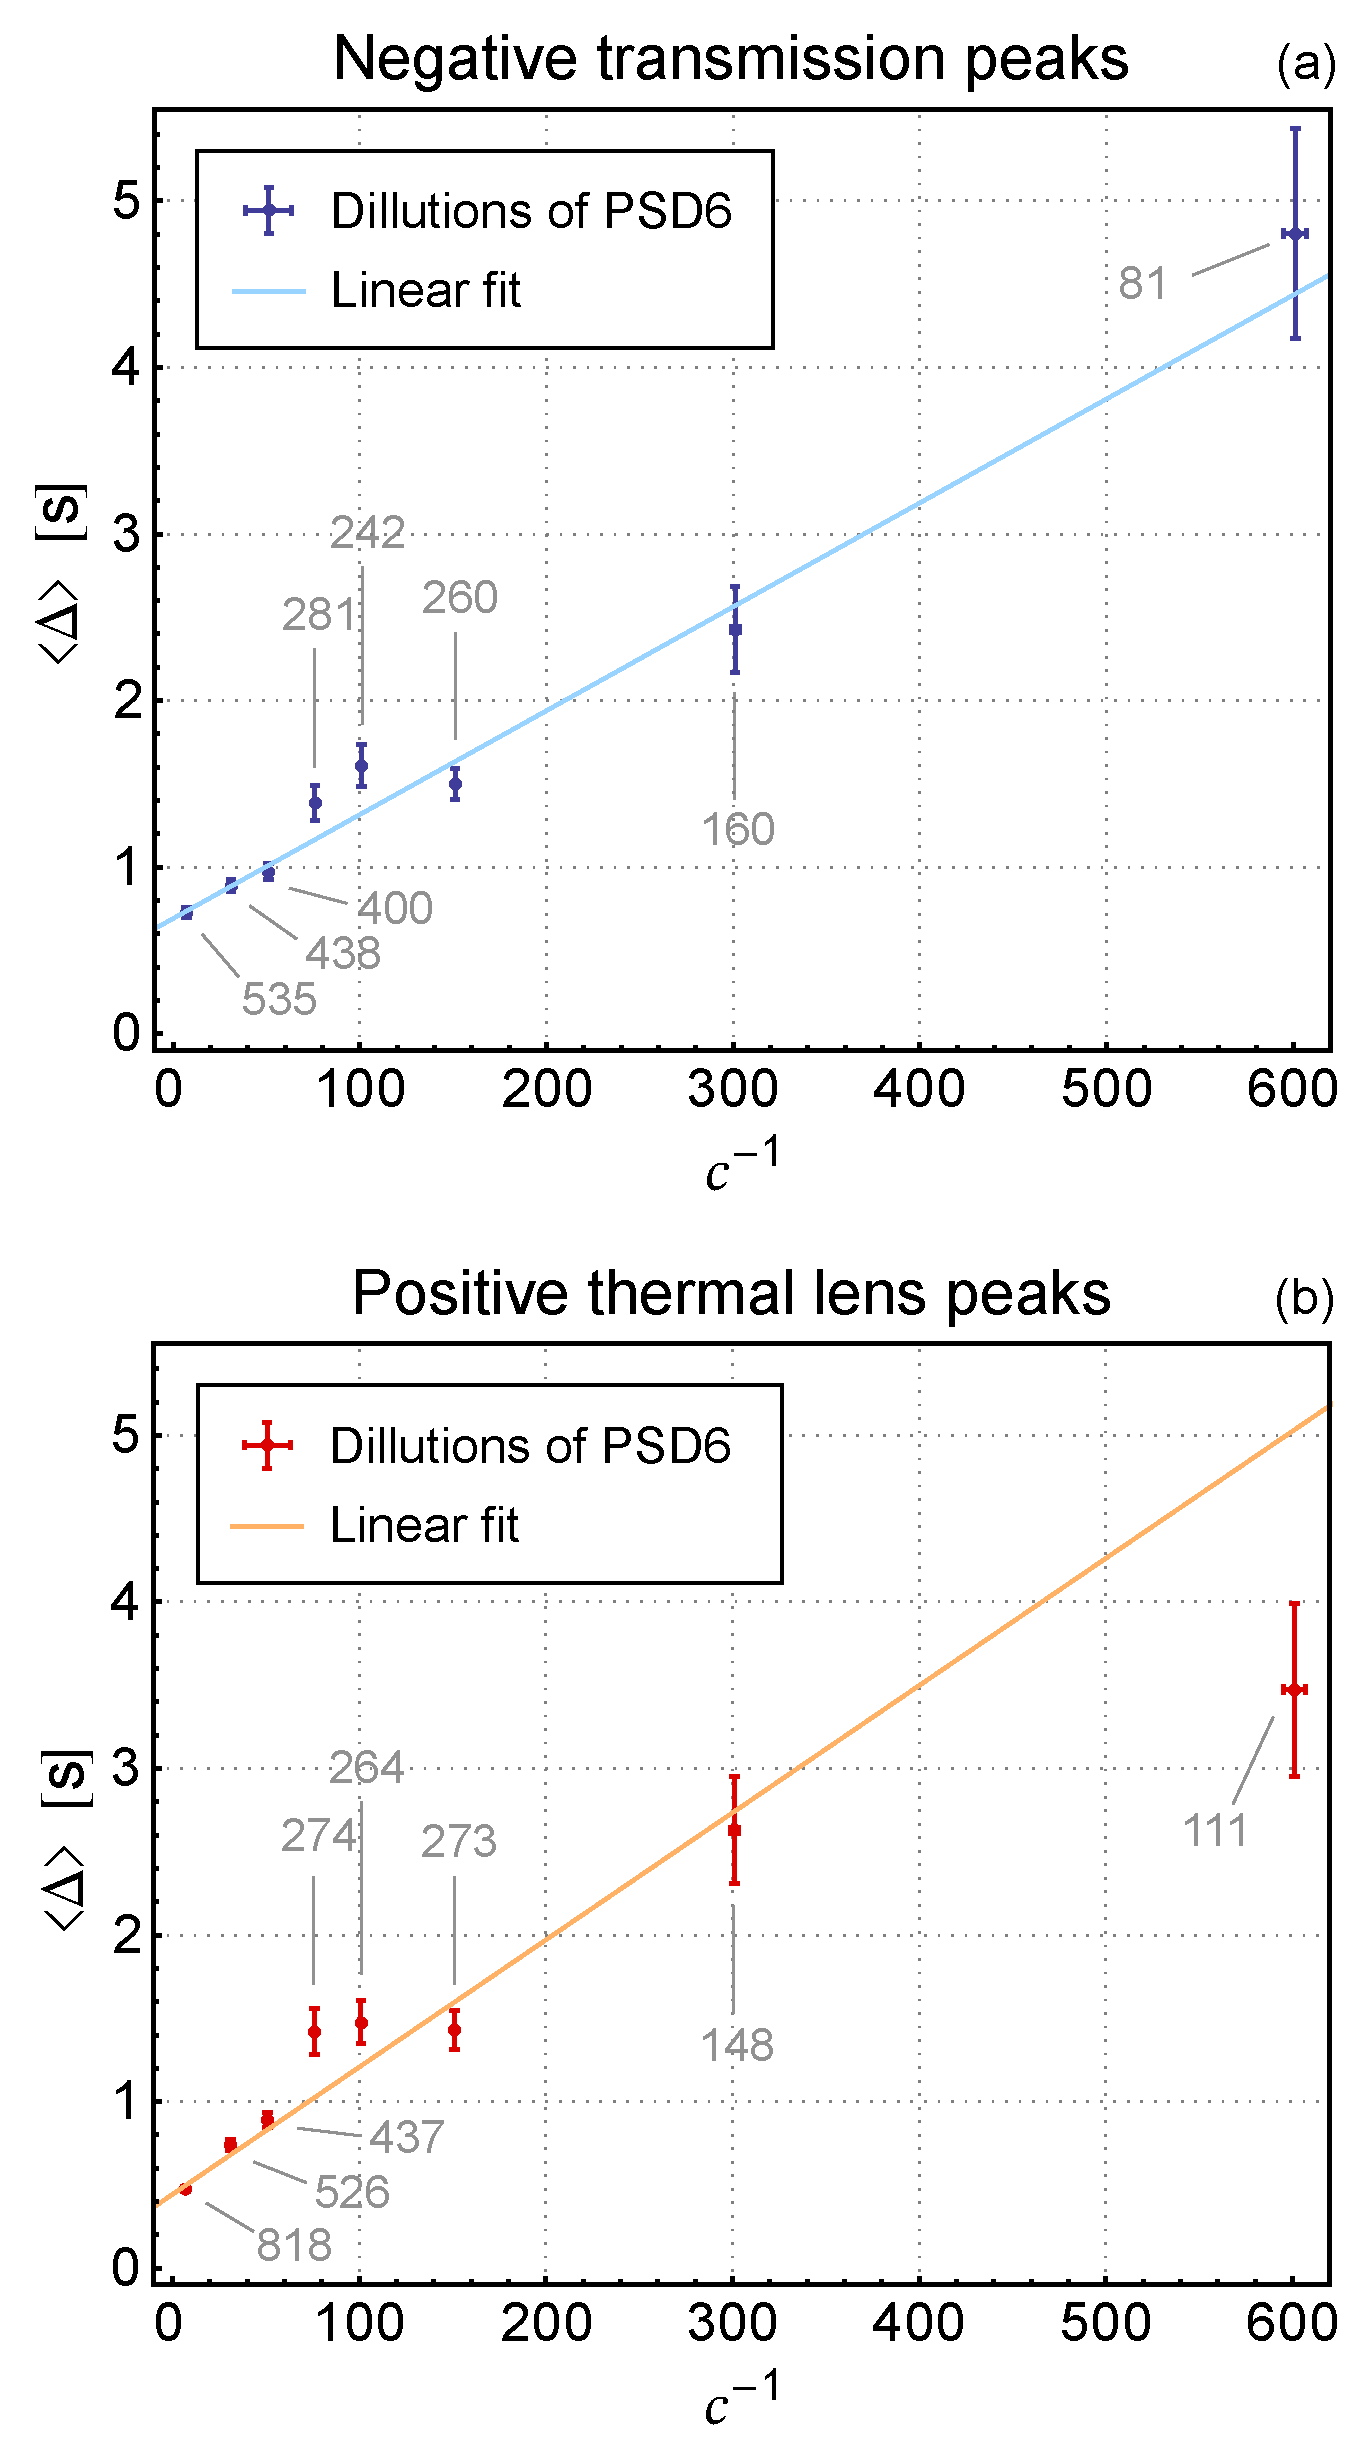
\includegraphics[width=.46\textwidth]{figures/InterarrivalTimes.pdf}
	\caption{Mean interarrival times of (a) peaks on transmission channel and (b) peaks on thermal lens channel obtained for serial dilutions of PSD6 on demineralized water, plotted against the reciprocal relative concentration $c$. Along with data points, the number of peaks detected for each dilution is indicated.}
	\label{fig:InterarrivalTimes}
\end{figure}

Under previous assumptions it is fairly simple to derive an expression for the parameter $b$ by explicit calculation of the probability of finding a particle in the sampling volume, obtaining
\begin{equation}
	b = 2 w_0 l u_\perp C,
\label{eq:bParamenter}
\end{equation}
where $l$ is the optical path of the cuvette, $2 w_0$ is the beam diameter, $u_\perp$ is the mean flow velocity in the direction transverse to the optical axis and $C$ is the absolute particle concentration (in units of number of particles per unit volume). Hence equation \ref{eq:bParamenter} corresponds to the flow of particles through the sampling volume. It should be mentioned that this expression is valid for a collimated beam in a uniform transverse flow, but it could be extended for focused beams and an almost arbitrary flow by considering an effective sampling volume and a mean transverse flow velocity. Thus, by knowing the sampling volume and the particle speed, the concentration $C$ can be estimated from the mean interarrival time $\left\langle \Delta \right\rangle$.

Consequently we performed an acquisition for a serial dilution of all master samples with polystyrene particles in demineralized water and measured $\left\langle \Delta \right\rangle$ for each iteration. Figure \ref{fig:InterarrivalTimes} shows the values of $\left\langle \Delta \right\rangle$ plotted against the reciprocal relative concentration $c^{-1}$ of each suspension for dilutions of the PSD6 master sample, indicating alongside the amounts of peaks detected on each iteration. It should be mentioned that in these experiments the flow velocity was determined only by the convective flow due to heat dissipation, thus varying for different concentrations because of the changes in the average absorbed energy. Nevertheless we observed a linear trend for both channels which we verified with a weighted linear regression. The adjusted slope is then associated to the sensitivity of our method, while the y-intercept is associated to $\Delta_{min}$ and limits our dynamic range since it corresponds to concentrations where the probability to find more than one particle in the beam is significant. In our case the measurable range of particle concentrations was limited to less than \SI{3000}{particles\per\milli\litre}.

Therefore by knowing the exact concentrations of each solution it is possible to obtain calibrations coefficients from the linear regression to finally measure absolute concentrations of absorbing and non-absorbing particles independently. For this purpose, an homogeneous and controlled flow profile, as it would be obtained with a proper installation of the system on the injection flowline, would be best suited since it provides a well-defined particle velocity and allows to tune the acquisition parameters to maximize the detection range and sensitivity.



\section{Conclusions}
\label{Conclusions}

We presented a system based on thermal lens effect and forward light scattering capable of performing online water quality measurements for continuous monitoring of both oil-in-water and suspended solids concentrations. The technique measures the bulk absorption of the sample due to dissolved hydrocarbons, which when tested with samples taken from an injection water facility showed a linear response that allows to measure oil concentrations with a minimum resolution of \SI{0.02}{\ppm} and a precision of at least \SI{5}{\percent}, limited mostly because of the signal fluctuations due to sample inhomogeneous composition.

The system can also detect both suspended solids and oil droplets in the size scale of the sampling volume by analyzing peaks in the signals due to single particles passing through the beams. For samples made from suspensions of dyed and undyed polystyrene spheres with diameters in the range of \SI{1}{}--\SI{10}{\micro\metre}, we showed that the system can distinguish each type of sphere since the peak height on each channel correlates with either the scattering or absorption cross section of the particle, allowing also to distinguish particles of different sizes from the peak height distribution. Suspended solids and oil droplets concentrations can be simultaneously measured after peak detection by calculating the mean interarrival time of the peaks on each channel, being limited by Poisson statistics validity, which in our case meant concentrations lesser than \SI{3000}{particles\per\milli\litre}.

For both type of samples studied we provide the calibration curves required for all concentration measurements. The method does not need sample preparation and results can be obtained from acquisitions \SI{200}{\second} long, making the system well suited for continuous on-line water quality monitoring. Incorporation into injection flowlines would also improve both particle concentration measurements reliability and precision by controlling the flow velocity through the sample. This configuration provides real-time measurements of the critical parameters that produces injectivity impairment.





\section*{Funding}
YPF Tecnología S.A.; Universidad de Buenos Aires (UBACYT 20020170100137BA); Agencia Nacional de Promoción Científica y Tecnológica (PICT 2015-1523).


\section*{Acknowledgements}
The authors also acknowledge support from the Universidad Nacional de Avellaneda.


\section*{Disclosures}
The authors declare no conflicts of interest.





% Bibliography
\bibliography{bibliography}

% Full bibliography added automatically for Optics Letters submissions; the following line will simply be ignored if submitting to other journals.
% Note that this extra page will not count against page length
\bibliographyfullrefs{bibliography}

%Manual citation list
%\begin{thebibliography}{1}
%\bibitem{Zhang:14}
%Y.~Zhang, S.~Qiao, L.~Sun, Q.~W. Shi, W.~Huang, %L.~Li, and Z.~Yang,
 % \enquote{Photoinduced active terahertz metamaterials with nanostructured
  %vanadium dioxide film deposited by sol-gel method,} Opt. Express \textbf{22},
  %11070--11078 (2014).
%\end{thebibliography}

% Please include bios and photos of all authors for aop articles
\ifthenelse{\equal{\journalref}{aop}}{%
\section*{Author Biographies}
\begingroup
\setlength\intextsep{0pt}
\begin{minipage}[t][6.3cm][t]{1.0\textwidth} % Adjust height [6.3cm] as required for separation of bio photos.
  \begin{wrapfigure}{L}{0.25\textwidth}
    \includegraphics[width=0.25\textwidth]{john_smith.eps}
  \end{wrapfigure}
  \noindent
  {\bfseries John Smith} received his BSc (Mathematics) in 2000 from The University of Maryland. His research interests include lasers and optics.
\end{minipage}
\begin{minipage}{1.0\textwidth}
  \begin{wrapfigure}{L}{0.25\textwidth}
    \includegraphics[width=0.25\textwidth]{alice_smith.eps}
  \end{wrapfigure}
  \noindent
  {\bfseries Alice Smith} also received her BSc (Mathematics) in 2000 from The University of Maryland. Her research interests also include lasers and optics.
\end{minipage}
\endgroup
}{}


\end{document}
